\documentclass[12pt]{exam}		%Doc : https://mirrors.ircam.fr/pub/CTAN/macros/latex/contrib/exam/examdoc.pdf
\printanswers					%Comment this line to hide the answers 
\usepackage[utf8]{inputenc}
\usepackage[T1]{fontenc}
\usepackage[french]{babel}      %Originally for french document, change to english or relevant language

\usepackage{amsmath,amssymb}
\usepackage{multicol}
\usepackage[dvipsnames]{xcolor}
\usepackage[shortlabels]{enumitem}
\usepackage{tikz}
	\usetikzlibrary{fadings}
	\usetikzlibrary{calc}
	
\usepackage{tkz-tab}
\usepackage{pgfplots}

%Format Header and footer
\pagestyle{headandfoot}
\header{\footnotesize Class\\Id number}{\Large\textbf{Name}}
\headrule
\footrule
\setlength{\columnsep}{0.25cm}
%\setlength{\columnseprule}{1pt}
\footer{}{Page \thepage}{}
%\extrafootheight{-2cm}

% Change section command behaviour
\usepackage{titlesec}
\titleformat{\section}[frame]{\Huge\bfseries\filright}{}{2mm}{\centering Chemistry 123 :\ }

% Add a watermark if answers are shown
%\ifprintanswers
%\usepackage{draftwatermark}
%\SetWatermarkColor{red!30}
%\SetWatermarkScale{5}
%\SetWatermarkText{Solution}     %Watermark text
%\fi

%Format the name of each exercise
\qformat{\textbf{Exercice \thequestion~:}\hfill}
\extrawidth{1.5cm}

\begin{document}
\section{Exam 2A}

\noindent The 60 pts exam consists of 5 questions and students have the whole class period to complete the exam.
Answers must be written in the box provided or else no credit is provided. Use the empty
space provided to do your work. A periodic table is provided at the end. Fill in your name along with your
student ID number.
\\

\noindent\textbf{Problem 1: Molarity - Acid/Base Reaction} Titration is a technique used to determine
an unknown of a solution. (12 pts)
\\
\begin{enumerate}[(a)]
\item To begin the experiment, 4 mL of 6.00 M NaOH stock solution is diluted to 240 mL.
  What is the new concentration?%
  \vspace{0.55in}
\item[]\tikz[baseline=1ex]\draw (0,0) rectangle (17cm,5ex);
\item Given the NaOH(aq) concentration from part a), NaOH(aq) is used to titrate acetic acid (CH$_3$COOH)
  by the chemical equation
  \begin{align*}
    \text{NaOH(aq)} + \text{CH$_3$COOH(aq)} \rightarrow \text{H$_2$O(l)} + \text{NaCH$_3$COO(aq)}
  \end{align*}

  Determine what volume of NaOH(aq) solution is needed to react with 0.300g CH$_3$COOH.
  \vspace{1.3in}
\item[]\tikz[baseline=1ex]\draw (0,0) rectangle (17cm,5ex);
\item Using the NaOH(aq) concentration from part a), you titrate 0.4274 g of unknown monoprotic acid,
  which only releases one hydrogen ion (H$^+$). To completely react all the acid, you used 35.00 mL of NaOH(aq)
  solution. What is the molar mass of the uknown acid? Hint: Recall the units for molar mass (g/mol).
  \vspace{1.25in}
\item[]\tikz[baseline=1ex]\draw (0,0) rectangle (17cm,5ex);
\end{enumerate}

\newpage

\noindent\textbf{Problem 2: Limiting Reagent} Small amounts of chlorine gas
can be generated in the laborator from the reaction of manganese(IV) oxide with
hydrochloric acd. The following is the balanced chemical equation. (12 pts)

 4 HCl(aq) +  MnO$_2$(s) $\rightarrow$ 2 H$_2$O(l) + MnCl$_2$(s) + Cl$_2$(g).

\\

\begin{enumerate}[(a)]
\item Given 42.7 g HCl(aq) and 67.0 g MnO$_2$(s), which one is the limiting
  reagent?
  \vspace{1.35in}
\item[]\tikz[baseline=1ex]\draw (0,0) rectangle (17cm,5ex);
\item What is the maximum amount of Cl$_2$(g) produced in g? This is also known
  as the theoretical yield.
  \vspace{1.35in}
\item[]\tikz[baseline=1ex]\draw (0,0) rectangle (17cm,5ex);
\item How much of the excess reagent in g is leftover?
  \vspace{1.35in}
\item[]\tikz[baseline=1ex]\draw (0,0) rectangle (17cm,5ex);
\item If 18.5 g of Cl$_2$(g) is collected, determine the percent yield.
  \vspace{1.3in}
\item[]\tikz[baseline=1ex]\draw (0,0) rectangle (17cm,5ex);
\end{enumerate}

\newpage

\noindent\textbf{Problem 3: Thermal Equilibrium} (12 pts)
\vspace{0.2in}

\noindent (a) True/False. If two objects are in contact and reach thermal equilibrium,
there is no flow of heat between the two objects.
\vspace{0.1in}

\tikz[baseline=1ex]\draw (0,0) rectangle (17cm,5ex);

\vspace{0.1in}
\noindent (b) 550.0g of Al metal block is heated to 500.0$^\circ$C and then, dropped into
1,000.g of water at 0$^\circ$C. The specific heats of water and Al are
4.184 J/(g $^\circ$C) and 0.9211 J/(g $^\circ$C), respectively. Determine the
final temperature at which the Al and water are in thermal equilibrium. Report to
4 significant figures.

\vspace{2.5in}

\tikz[baseline=1ex]\draw (0,0) rectangle (17cm,5ex);
\\

\noindent (c) Describe using illustrations and/or equations to show how thermal equilibrium
is achieved. Include the initial and final states of the Al and water.
\\

\tikz[baseline=1ex]\draw (0,0) rectangle (17.5cm,42ex);

\newpage

\noindent\textbf{Problem 4: Charles' Law} Given a fixed amount of gas at constant
pressure. Answer the following questions. (12 pts)

\begin{enumerate}[(a)]
\item Starting from the ideal gas law $PV = nRT$. Show how you can arrive at Charles'
  law. Include all steps to receive full credit.
\item[]\tikz[baseline=1ex]\draw (0,0) rectangle (17cm,15ex);  
\item If a sample of chlorine gas occupies 50.0mL at 100.$^\circ$C, what is its
  volume at 25.0$^\circ$C?
  \vspace{1.5in}
\item[]\tikz[baseline=1ex]\draw (0,0) rectangle (17cm,5ex);
\item Calculate the temperature (in Celsius) when 2.00L at 21.0$^\circ$C is
  compressed to 1.00L.
  \vspace{1.5in}
\item[]\tikz[baseline=1ex]\draw (0,0) rectangle (17cm,5ex);
\item Draw the graph of the relationship between volume (V) and temperature (T)
  for an ideal gas. Describe the relationship.
\item[]\tikz[baseline=1ex]\draw (0,0) rectangle (17cm,30ex);
\end{enumerate}

\newpage

\noindent\textbf{Problem 5: Hess's Law} Given the overall reaction:
(12 pts)

3 Fe$_2$O$_3$(s) + CO(g) $\rightarrow$ 2 Fe$_3$O$_4$(s) + CO$_2$(g)
\\

Given the folowing data:

Fe$_2$O$_3$(s) + 3 CO(g) $\rightarrow$ 2 Fe(s) + 3CO$_2$(g) $\Delta H = -23.44 \text{ kJ/mol}$

Fe$_3$O$_4$ + CO(g) $\rightarrow$ 3 FeO(s) + CO$_2$(g) $\Delta H = +21.79 \text{ kJ/mol}$

Fe(s) + CO$_2$(g) $\rightarrow$ FeO(s) + CO(g) $\Delta H = -10.94 \text{ kJ/mol}$

\vspace{2.5in}

\noindent (a) Determine the enthalpy for the overall reaction:

3 Fe$_2$O$_3$(s) + CO(g) $\rightarrow$ 2 Fe$_3$O$_4$(s) + CO$_2$(g)

\tikz[baseline=1ex]\draw (0,0) rectangle (17cm,5ex);

\vspace{0.25in}

\noindent (b) Is the overall reaction exothermic or endothermic?

\tikz[baseline=1ex]\draw (0,0) rectangle (17cm,5ex);

\vspace{0.25in}

\noindent (c) Given your answer in part (b), sketch the energy diagram
for the overall reaction. Include in your diagram the  relative energies of the reactants
(Fe$_2$O$_3$, CO) and products (Fe$_3$O$_4$, CO$_2$), activation energy ($E_A$),
and energy difference ($\Delta E$).
\\

\tikz[baseline=1ex]\draw (0,0) rectangle (17.5cm,32ex);

\newpage

\appendix

\section{Apppendix 2 - Formulas and Constants}

\begin{align*}
  \text{percent yield} & = \frac{\text{Actual}}{\text{Theoretical}}\times 100\% \\
  M_1V_1 & = M_2V_2 \\
  P_1V_1 & = P_2V_2 \\
  \frac{V_1}{T_1} & = \frac{V_2}{T_2} \\
  \frac{V_1}{n_1} & = \frac{V_2}{n_2} \\
  q & = mc\Delta T
\end{align*}

\begin{center}
  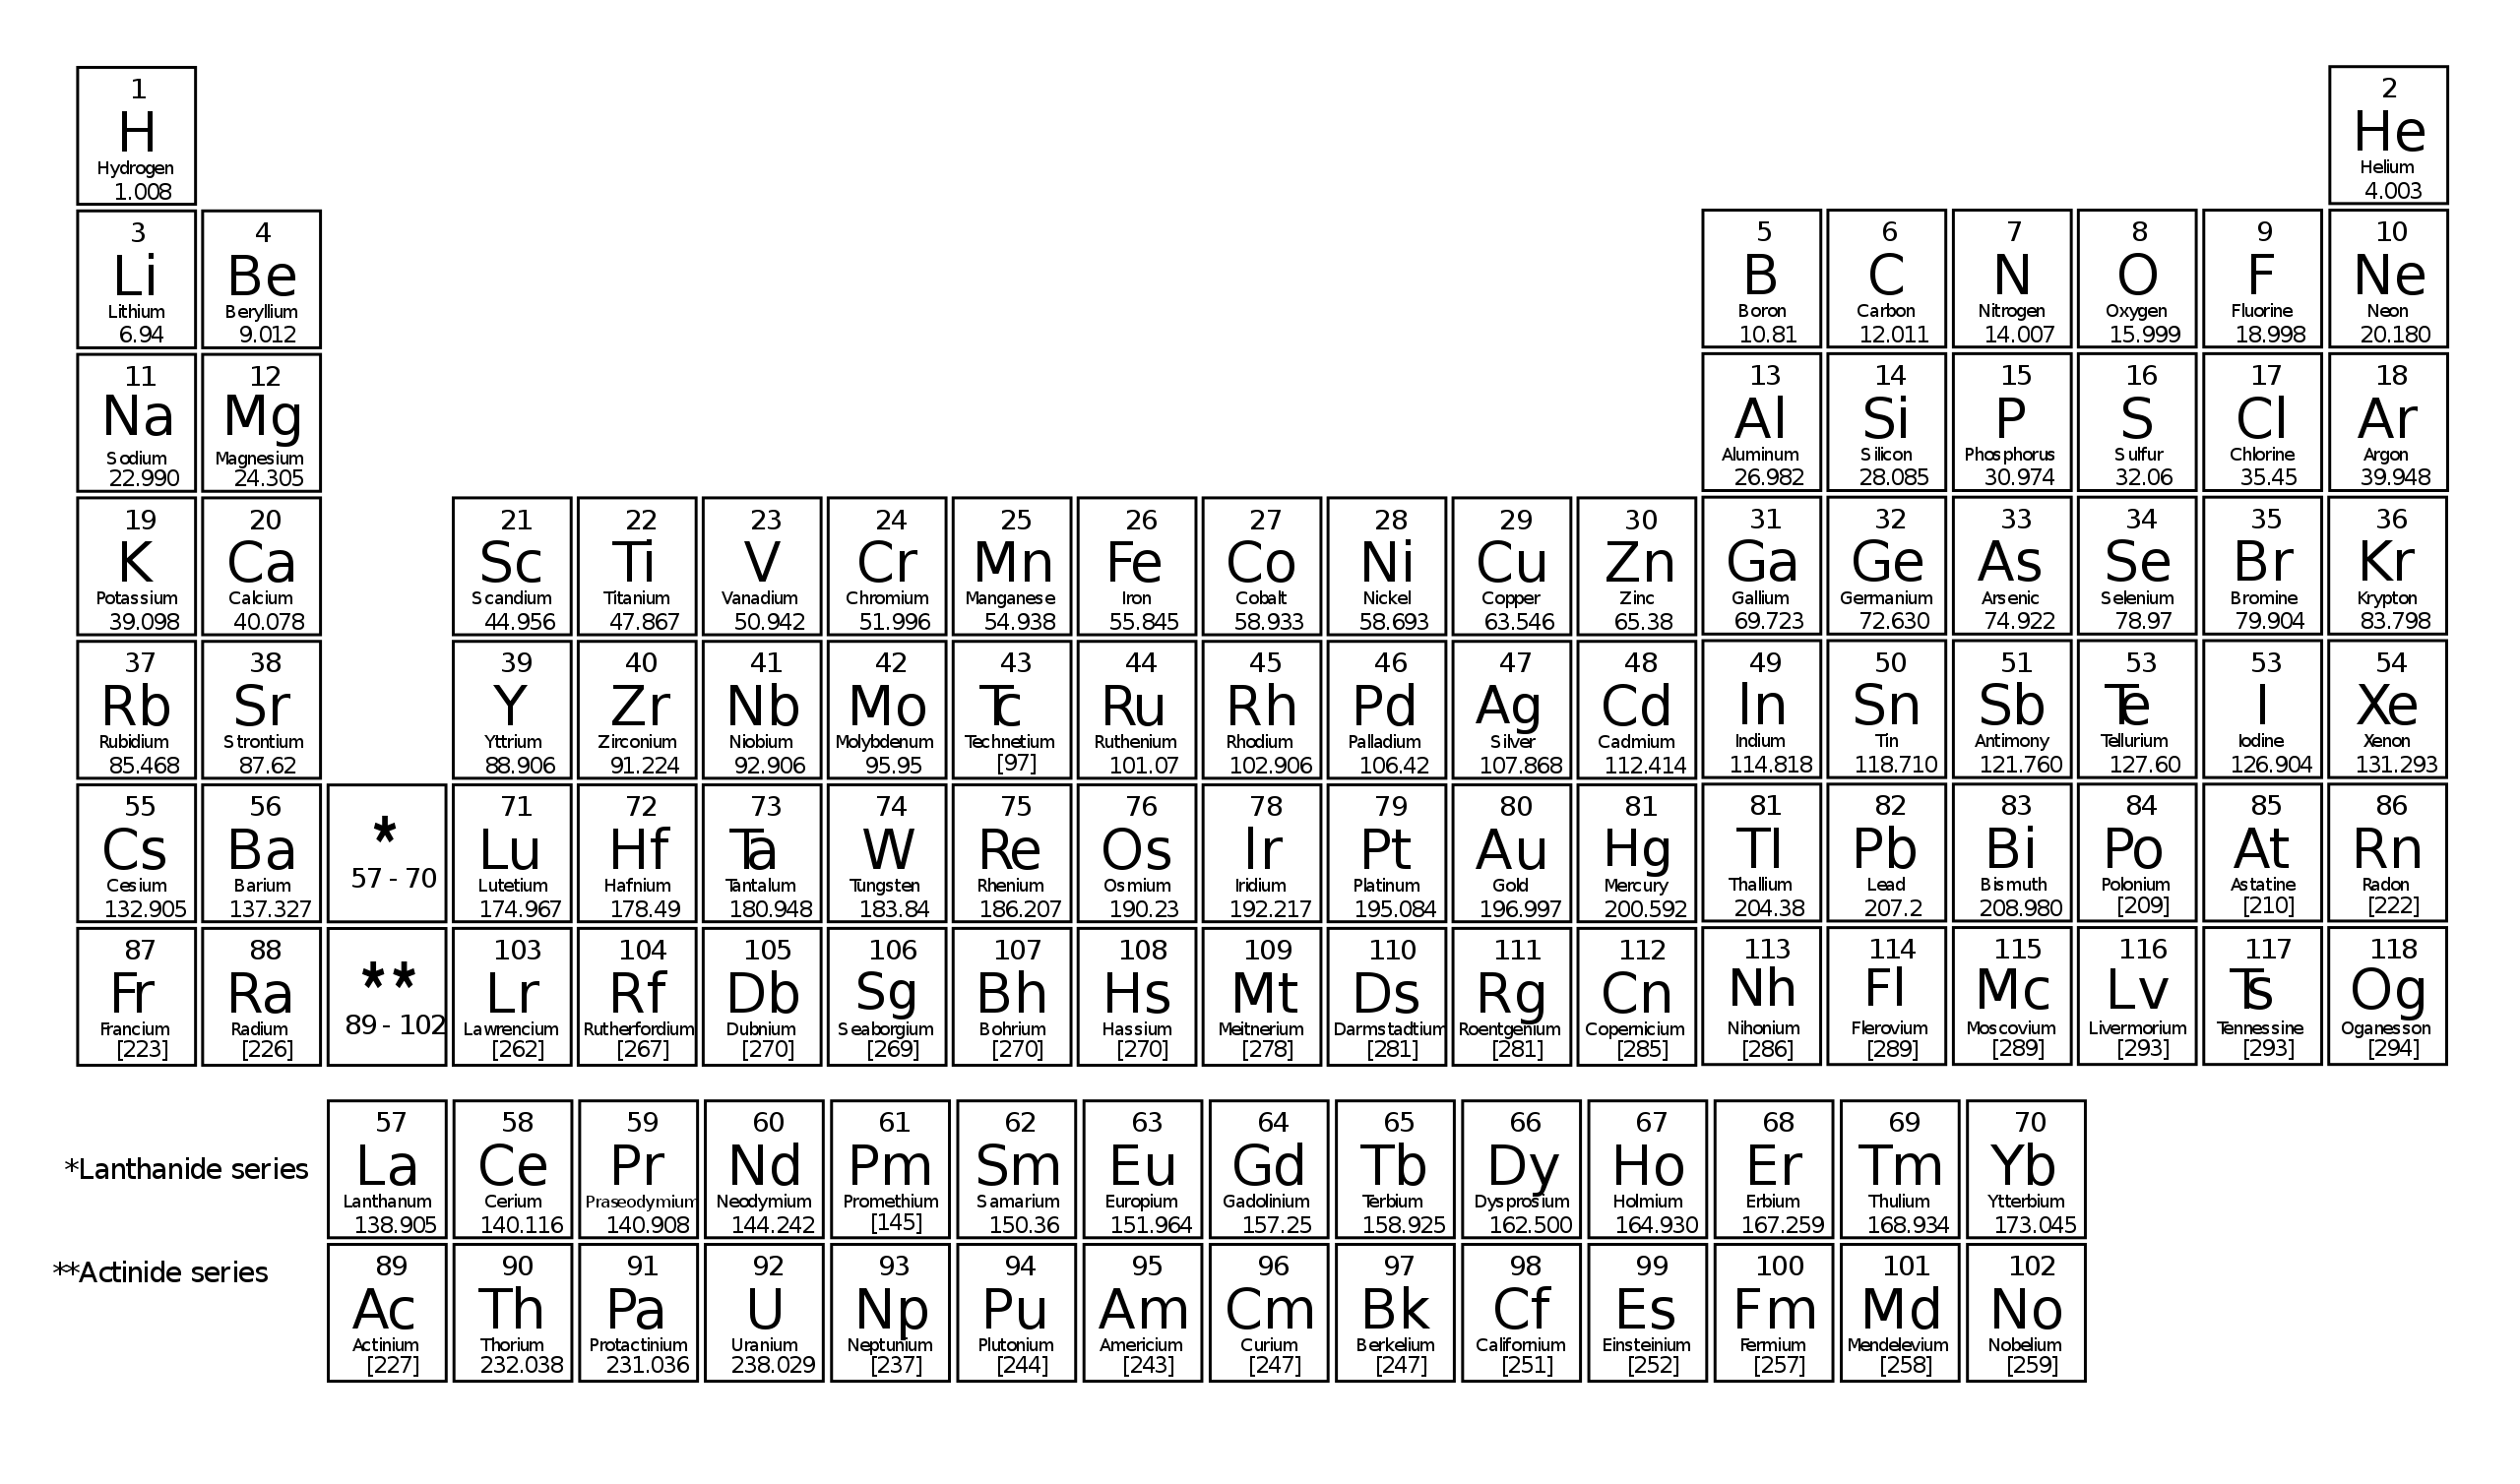
\includegraphics[scale=0.26,angle=90]{periodic_table}
\end{center}

\end{document}
